\documentclass{article}
\usepackage{fancyhdr}
\usepackage{extramarks}
\usepackage{amsmath}
\usepackage{amsthm}
\usepackage{amsfonts}
\usepackage{tikz}
% \usepackage[fontset=ubuntu]{ctex}
\usepackage[UTF8, scheme=plain, punct=plain, zihao=false]{ctex}
\usepackage[shortlabels]{enumitem}
\usetikzlibrary{automata,positioning}
\usepackage{algorithm}
\usepackage{algpseudocode}
\usepackage{algpascal}
% \usepackage{algorithmic}
\usepackage{float}  
\usepackage{lipsum}


% \makeatletter  
% \newif\if@restonecol  
% \makeatother  
% \let\algorithm\relax  
% \let\endalgorithm\relax  
% \usepackage[linesnumbered,ruled,vlined]{algorithm2e}%[ruled,vlined]{ 

\renewcommand{\algorithmicrequire}{\textbf{Input:}}  % Use Input in the format of Algorithm  
\renewcommand{\algorithmicensure}{\textbf{Output:}} % Use Output in the format of Algorithm
\newcommand{\True}{\textbf{true}}
\newcommand{\False}{\textbf{false}}
\usepackage{graphics}
\usepackage{epsfig}
\usepackage{indentfirst}
%
% Basic Document Settings
%
% 算法跨页
\makeatletter
\newenvironment{breakablealgorithm}
  {% \begin{breakablealgorithm}
%   \begin{center}
     \refstepcounter{algorithm}% New algorithm
     \hrule height.8pt depth0pt \kern2pt% \@fs@pre for \@fs@ruled
     \renewcommand{\caption}[2][\relax]{% Make a new \caption
      {\raggedright\textbf{\ALG@name~\thealgorithm} ##2\par}%
      \ifx \relax##1\relax % #1 is \relax
         \addcontentsline{loa}{algorithm}{\numberline{\thealgorithm}##2}%
      \else % #1 is not \relax
         \addcontentsline{loa}{algorithm}{\numberline{\thealgorithm}##1}%
      \fi
      \kern2pt\hrule\kern2pt
     }
  }{% \end{breakablealgorithm}
     \kern2pt\hrule\relax% \@fs@post for \@fs@ruled
%   \end{center}
  }
\makeatother


\topmargin=-0.45in
\evensidemargin=0in
\oddsidemargin=0in
\textwidth=6.5in
\textheight=9.0in
\headsep=0.25in

\linespread{1.1}

\pagestyle{fancy}
\lhead{\hmwkAuthorName}
\chead{\hmwkClass\ \hmwkTitle}
\rhead{\firstxmark}
\lfoot{\lastxmark}
\cfoot{\thepage}

\renewcommand\headrulewidth{0.4pt}
\renewcommand\footrulewidth{0.4pt}

% \setlength\parindent{0pt}

%
% Create Problem Sections
%

\newcommand{\enterProblemHeader}[1]{
    \nobreak\extramarks{}{Problem \arabic{#1} continued on next page\ldots}\nobreak{}
    \nobreak\extramarks{Problem \arabic{#1} (continued)}{Problem \arabic{#1} continued on next page\ldots}\nobreak{}
}

\newcommand{\exitProblemHeader}[1]{
    \nobreak\extramarks{Problem \arabic{#1} (continued)}{Problem \arabic{#1} continued on next page\ldots}\nobreak{}
    \stepcounter{#1}
    \nobreak\extramarks{Problem \arabic{#1}}{}\nobreak{}
}

\setcounter{secnumdepth}{0}
\newcounter{partCounter}
\newcounter{homeworkProblemCounter}
\setcounter{homeworkProblemCounter}{1}
\nobreak\extramarks{Problem \arabic{homeworkProblemCounter}}{}\nobreak{}

%
% Homework Problem Environment
%
% This environment takes an optional argument. When given, it will adjust the
% problem counter. This is useful for when the problems given for your
% assignment aren't sequential. See the last 3 problems of this template for an
% example.
%
\newenvironment{homeworkProblem}[1][-1]{
    \ifnum#1>0
        \setcounter{homeworkProblemCounter}{#1}
    \fi
    \section{\huge{Problem} \arabic{homeworkProblemCounter}}
    \setcounter{partCounter}{1}
    \enterProblemHeader{homeworkProblemCounter}
}{
    \exitProblemHeader{homeworkProblemCounter}
}

%
% Homework Details
%   - Title
%   - Due date
%   - Class
%   - Section/Time
%   - Instructor
%   - Author
%

\newcommand{\hmwkTitle}{第2次作业}
\newcommand{\hmwkDueDate}{Sep. 19, 2021}
\newcommand{\hmwkClass}{计算机算法设计与分析}
 \newcommand{\hmwkClassTime}{Section A}
 \newcommand{\hmwkClassInstructor}{主讲教师:卜东波}
\newcommand{\hmwkAuthorName}{张倩倩 202128007329011}
% \newcommand{\hmwkAuthorName}{\textbf{202028013229110}}

%
% Title Page
%

\title{
    \vspace{2in}
    \textmd{\textbf{\Huge{\hmwkClass}
    \\ \Large{\hmwkTitle}}}\\
    % \normalsize\vspace{0.1in}\small{Due\ on\ \hmwkDueDate\ at 3:10pm}\\
    \vspace{0.1in}\large{\textit{\hmwkClassInstructor\ \hmwkClassTime}}
    \vspace{3in}
}

\author{\Large{\textbf{张倩倩}}\\\textbf{202128007329011}}
% \hmwkAuthorName}
\date{}

\renewcommand{\part}[1]{\textbf{\large Part \Alph{partCounter}}\stepcounter{partCounter}\\}

%
% Various Helper Commands
%

% Useful for algorithms
\newcommand{\alg}[1]{\textsc{\bfseries \footnotesize #1}}

% For derivatives
\newcommand{\deriv}[1]{\frac{\mathrm{d}}{\mathrm{d}x} (#1)}

% For partial derivatives
\newcommand{\pderiv}[2]{\frac{\partial}{\partial #1} (#2)}

% Integral dx
\newcommand{\dx}{\mathrm{d}x}

% Alias for the Solution section header
\newcommand{\solution}{\textbf{\large Solution}}

% Probability commands: Expectation, Variance, Covariance, Bias
\newcommand{\E}{\mathrm{E}}
\newcommand{\Var}{\mathrm{Var}}
\newcommand{\Cov}{\mathrm{Cov}}
\newcommand{\Bias}{\mathrm{Bias}}


\begin{document}
\alglanguage{pseudocode}
% \setmainfont{SimSun} % 宋体
\maketitle

\pagebreak
\begin{homeworkProblem}
\textbf{\large{对应sep发布的作业题1:Money robbing   A robber is planning to rob houses along a street. Each house has a certain amount of money stashed, the only constraint stopping you from robbing each of them is that adjacent houses have security system connected and it will automatically contact the police if two adjacent houses were broken into on the same night.
		1.	Given a list of non-negative integers representing the amount of money of each house, determine the maximum amount of money you can rob tonight without alerting the police.
		2.	What if all houses are arranged in a circle?
}}

\subsection{the optimal substructure and DP equation}
用 \textit{dp}[i] 表示前i间房屋能偷窃到的最高总金额。如果只有一间房屋,则可以偷窃到最高总金额就是该间房屋里的金钱:dp[0]=nums[0]。如果只有两间房屋(隐藏条件:两间房屋相邻不能同时偷窃,只能偷窃其中的一间房屋)所以偷窃到最高总金额为两个房间金钱中钱最多的那个房间dp[1]=max(nums[0],nums[1])。如果房屋数量大于两间,有两个选项:偷或者不偷。如果偷第m间房(m>2)那就不能偷窃m-1间房,偷窃总金额为前 m-2间房屋的最高总金额与第 m 间房屋的金额之和,dp[i-2]+nums[i]。如果不偷,则总金额为前m-1间房屋的最高总金额dp[i-1]。在两个选项中选择大的那项,即为前m间房屋能偷窃到的最高总金额。最终返回\textit{dp}[n-1],其中 n 是数组的长度。则对应的DP方程为:
\begin{equation}
	\mathrm{dp}[\mathrm{i}]= \begin{cases}\text { nums[0] } & \mathrm{i}=0\\ \text { max(nums[0],nums[1]) } & \mathrm{i}=1 \\ \text { dp[i-2]+nums[i],dp [i-1] } & 1<i<\text { nums.length}\end{cases}
\end{equation}
\subsection{\solution}

\begin{breakablealgorithm}
	\caption{求解打家劫舍}
	\begin{algorithmic}[1]
		\Require{一个代表每个房屋存放金额的非负整数数组。}%\Comment{A is ..., B is ...}
		\Ensure{一夜之内能够偷窃到的最高金额。}%\Comment{C is ..., D is ...}
		
		
		\Function{Moneyrob}{nums}
		%\Comment{$如果...就...$}
		\State if(n=0)   \qquad\qquad //如果房间数为0,那么就直接返回盗窃的金额为0
		\State \qquad return 0
		\State end if
		\State if(n=1)   \qquad\qquad //如果房间数为1,则最大收益为第一间房间内藏有的全部金额
		\State  \qquad return nums[0]  
		\State end if
		\State //创建dp数组,用来记录状态
		\State//初始化dp[0]和dp[1]
		\State dp[0] = nums[0]
		\State dp[1] = max(nums[0], nums[1])
		\State //根据dp公式,依次更新dp[i]
		\State for (int i = 2; i < n; i++)\qquad\qquad//n为数组长度
		\State \qquad dp[i] = max(dp[i - 2] + nums[i], dp[i - 1])
		\State end for
		\State return dp[n - 1]\qquad\qquad//最终返回最大收益
		\EndFunction
	\end{algorithmic}
\end{breakablealgorithm}
\subsection{Proof of the correctness}
举以下例子来证明算法的正确性:
假设从数组\{1,2,3,1\}中寻找一夜之内能够偷窃到的最高金额(即偷窃到的最高金额 = 1 + 3 = 4 。)
\begin{figure}[H]
	\centering                                      %图片居中
	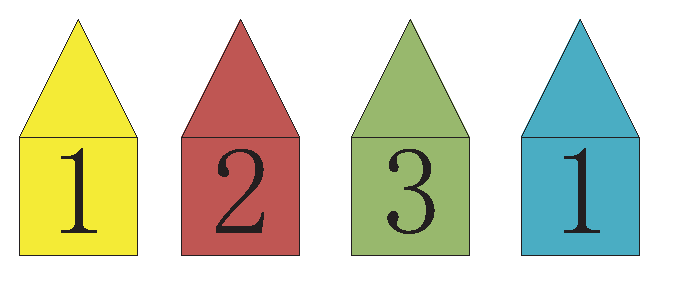
\includegraphics[width=.4\textwidth]{绘图1.eps}    %xx.eps是图片文件的相对路径
	\caption{待偷窃房屋}                                  %图片的标题
	\label{img}                                     %此处的label相当于一个图片的专属标志,目的是方便上下文的引用
\end{figure}
\begin{flushleft} 
	1.偷窃第一间房屋:dp[0]=nums[0]=1,最大金额为1。
\\ 2.偷窃前两间房屋:dp[1]=max(nums[0], nums[1])=2,最大金额为2。
\\3.偷窃前三间房屋:dp[2]=max(dp[0]+nums[2], dp[1])=max(1+3,2)=4,最大金额为4。max(偷窃前2间房屋的最高金额,第1间房屋+第3间房屋的总金额)
\\4.偷窃前4间房屋:dp[3]=max(dp[1]+nums[3], dp[2])=max(2+1,4)=4,最大金额为4。max(偷窃前3间房屋的最高金额,第2间房屋+第4间房屋的总金额)
\\5.返回dp[n-1]=dp[3]=4。和预测的结果一样。
\end{flushleft}

\subsection{Analysis of Complexity}
   \textbf{时间复杂度}$O(n)$。从0到n-1依次更新每个状态(此处的n为数组长度,即房屋总数)所以时间复杂度为$O(n)$。
   \textbf{空间复杂度}$O(n)$。因为使用了一个长度为n的数组记录dp[i]。
   	\begin{flushleft} 
	第二小问:如果所有的房子都排成一个圆圈呢?
   
   	 \end{flushleft}
   	\begin{figure}[H]
   		\centering                                      %图片居中
   		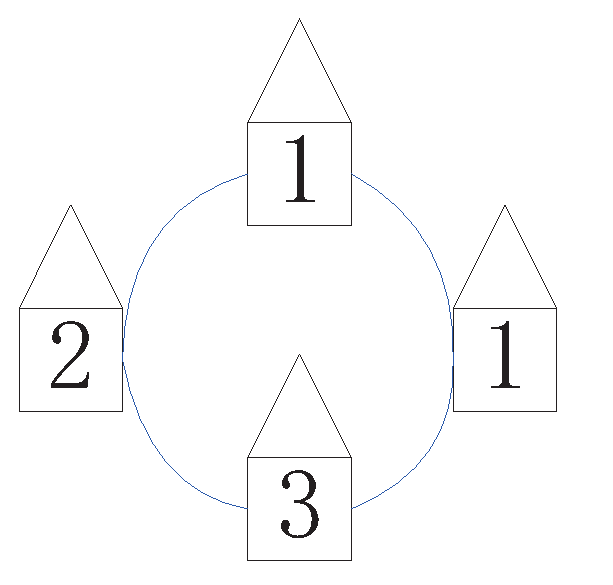
\includegraphics[width=0.4\textwidth]{绘图8.eps}    %xx.eps是图片文件的相对路径
   		\caption{环形房屋}                                  %图片的标题
   		\label{img}                                     %此处的label相当于一个图片的专属标志,目的是方便上下文的引用
   	\end{figure}
  \subsection{the optimal substructure and DP equation}
   	只一间房,偷该房可得到最高总金额。只两间房,两间房相邻,不能同时偷,选其中金额高偷。如果房屋数量大于两间,第一间和最后一间房不能同时偷。如果偷了第一间就不能偷最后一间房,偷的范围是第一间房到最后第二间房屋;如果偷了最后一间房,则不能偷第一间,偷的范围是第二间房到最后一间房。假设数组nums 的长度为n。如果不偷最后一间房,偷的下标范围是[0,n−2];如果不偷第一间房,偷的下标范围是[1,n−1]。然后比较两个中那个偷盗的更多,就是偷的最大金额。
   	假设偷的下标范围是[start,end],用dp[i] 表示在下标范围[start,i] 内可以偷到的最高总金额,dp方程为:
   	$$
   	d p[i]=\max (d p[i-2]+\text { nums }[i], d p[i-1])
   	$$
   
   	
   	 \begin{flushleft} 
   	1.求出第一家到倒数第二家的最大钱财数量
   	2.求出第二家到最后一家的最大钱财数量
   	3.求两者的较大值
   	即分别取(start,end)=(0,n−2) 和(start,end)=(1,n−1) 进行计算,取两个dp[end] 中的最大值,即为下标范围[start,end]内可以偷到的最高总金额。
   \end{flushleft} 
	特殊情况:
$$
\begin{cases}d p[\text i]=\text { nums }[\text { start }] & \text { 只有一间 } \\ d p[\text i]=\max (\text { nums }[\text { start }], \text { nums }[\text { start }+1]) & \text { 只有两间房屋 }\end{cases}
$$
   \subsection{\solution}
   
   \begin{breakablealgorithm}
   	\caption{求解环形打家劫舍}
   	\begin{algorithmic}[1]
   		\Require{一个代表每个房屋存放金额的非负整数数组。}%\Comment{A is ..., B is ...}
   		\Ensure{一夜之内能够偷窃到的最高金额。}%\Comment{C is ..., D is ...}
   		
   		
   		\Function{rob}{nums}
   		%\Comment{$如果...就...$}
   		\State//取输入数组长度n
   		\State if(n=1)   \qquad\qquad //如果只有一家
   		\State \qquad return nums[0]//直接返回这家的金钱;
   		\State end if
   		\State if(n=2)   \qquad\qquad //如果有两家
   		\State  \qquad  return max(nums[0], nums[1])//返回两家中金额最多的
   		\State end if
   		\State //如果有两家以上
   		\State  return max(robRange(nums, 0, length - 2), robRange(nums, 1, length - 1))//分别取(start,end)=(0,n−2) 和(start,end)=(1,n−1) 进行计算,取两个dp[end] 中的最大值返回
   		\EndFunction
   		\Function{robRange}{nums, start, end}
   		%\Comment{$如果...就...$}
   		\State first = nums[start], second = max(nums[start], nums[start + 1])
   		\State for (int i = start + 2; i <= end; i++) 
   		\State \qquad temp = second
   		\State \qquad second = max(first + nums[i], second)
   		\State \qquad first = temp
   		\State end for
   		\State return second
   		\EndFunction
   	\end{algorithmic}
   \end{breakablealgorithm}
   \subsection{Proof of the correctness}
   如果只有一间房,则偷该房可得到最高总金额。如果只有两间房,则由于两间房相邻,不能同时偷,只能偷其中的一间房,选择其中金额较高的房进行偷就是最高总金额。如果房屋数量大于两间,第一间房和最后一间房不能同时偷。如果偷了第一间房就不能偷最后一间房,偷的范围是第一间房到最后第二间房屋;如果偷了最后一间房,则不能偷第一间房,偷的范围是第二间房到最后一间房。进行计算,取两个dp[end] 中的最大值返回。
   
   
   
\subsection{Analysis of Complexity}
\textbf{时间复杂度}$O(n)$。
\textbf{空间复杂度}$O(n)$。
\end{homeworkProblem}

\pagebreak
\begin{homeworkProblem}
	\textbf{\large{对应sep发布的作业题2:Largest Divisible Subset    Given a set of distinct positive integers, find the largest subset such that every pair (Si, Sj) of elements in this subset satisfies: Si\%Sj = 0 or Sj\%Si = 0.Please return the largest size of the subset.Note:	Si\%Sj = 0 means that Si  is divisible by Sj.
	}}
	
	\subsection{the optimal substructure and DP equation}
	dp[i] 表示在输入数组nums 升序排列的前提下,以 nums[i] 为最大整数的整除子集的大小。存在2种情况:如果在i之前找不到符合nums[i]\%nums[j]==0的位置j,那么nums[i]不能接在i之前的数后面,只能自己独立作为整除子集的第一个数,此时dp[i]=1。如果在i之前能够找到符合条件的j,则取符合条件的dp[j]的最大值。表示如果找到以nums[i]结尾的最长子集,将nums[i]接到符合条件的最长nums[j]后面。此时dp[i]=dp[j]+1。则对应的DP方程为:
	\begin{equation}
		d p[i]= \begin{cases}\max (\mathrm{dp}[\mathrm{i}], \mathrm{dp}[\mathrm{j}]+1)& \text { if nums[i]\%nums }[j]==0 \\   \\ 1 & \text { if nums[i]\%nums }[j] !=0 \end{cases}
	\end{equation}
	\subsection{\solution}
	\begin{breakablealgorithm}
		\caption{最大整除子集}
		\begin{algorithmic}[1]
			\Require{无重复正整数组成的集合nums}%\Comment{A is ..., B is ...}
			\Ensure{最大整除子集res}%\Comment{C is ..., D is ...}
			
			\Function{largestDivisibleSubset}{nums}
			\State len = nums.size() \qquad \qquad //取输入数组的长度
			\State sort(nums.begin(),nums.end()) \qquad \qquad//用sort函数升序排序,算法复杂度为$O(nlogn)$
			\State //找出最大子集、最大子集中的最大整数
			\State //初始化长度为len长的dp,初始化值dp[i]=1
			\State maxSize = 1\qquad \qquad//最大子集尺寸赋初始值为1
			\State maxVal = dp[0];\qquad \qquad//最大子集中的最大整数初始值为dp[0]
			\State for (int i = 1; i < len; i++)
			\State \qquad for (int j = 0; j < i; j++)
			\State \qquad \qquad if (nums[i] \% nums[j]==0)\qquad \qquad//如果存在整除关系,取所有符合条件的dp的最大值
			\State \qquad \qquad\qquad dp[i] = max(dp[i], dp[j] + 1)
			\State \qquad \qquad end if
			\State \qquad end for
			\State \qquad if(dp[i] > maxSize)\qquad \qquad//如果找到了,更新两个最大值
			\State \qquad \qquad maxSize = dp[i]
			\State  \qquad \qquad maxVal = nums[i]
			\State \qquad end if
			\State end for
			\State //然后倒着遍历得到最大整除子集
			\State if (maxSize == 1)\qquad \qquad//如果最大整除子集大小为1,则直接返回nums[0]
			\State  \qquad res.push\_back(nums[0])
			\State \qquad return res
			\State end if
			\State for (int i = len - 1; i >= 0 \&\& maxSize > 0; i--) \qquad \qquad//倒着遍历
			\State  \qquad if (dp[i] == maxSize \&\& maxVal \% nums[i] == 0)\qquad//满足条件,就装入,直到全部遍历完
			\State  \qquad \qquad res.push\_back(nums[i])
			\State \qquad \qquad maxVal = nums[i]
			\State \qquad \qquad maxSize--
			\State \qquad end if
			\State end for
			\State return res\qquad \qquad//返回最大整除子集
			
			\EndFunction
		\end{algorithmic}
	\end{breakablealgorithm}
	
	
	\subsection{Proof of the correctness}
	
	\begin{flushleft} 
		本题中定义dp[i]表示输入数组nums升序排序的前提下,以nums[i]为最大整数的整除子集的大小,初始化时,dp[i]=1,(其中i=0,1...n-1)循环遍历nums[j],如果满足nums[i] \% nums[j]==0,则说明nums[i]可以扩充在以nums[j]为最大整数的整数子集成为一个更大的整数子集。找到最大子集、最大子集中的最大整数之后,倒序遍历数组dp,直到找到dp[i]=maxSize 为止,把此时对应的nums[i] 加入结果集,此时 maxVal=nums[i];然后将 maxSize 的值减1,继续倒序遍历找到 dp[i]=maxSize,且 nums[i] 能整除 maxVal 的i为止,将此时的nums[i] 加入结果集,maxVal 更新为此时的 num[i];重复上述操作,直到 maxSize 的值变成0,此时的结果集即为目标子集。
		\\举个例子进行详细说明:
	\end{flushleft} 
	\begin{figure}[H]
		\centering                                      %图片居中
		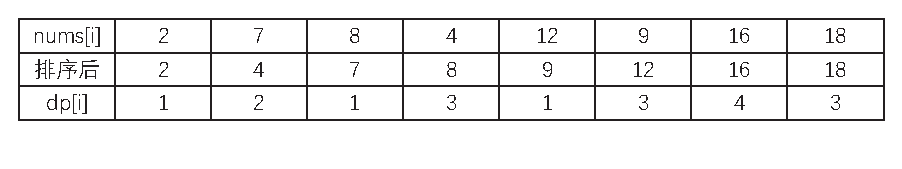
\includegraphics[width=1\textwidth]{绘图7.eps}    %xx.eps是图片文件的相对路径
		\caption{排序并计算dp[i]后的结果表}                                  %图片的标题
		\label{img}                                     %此处的label相当于一个图片的专属标志,目的是方便上下文的引用
	\end{figure}

	\begin{flushleft} 
		倒序遍历求得最大整除子集:
		\\1.根据dp结果(表格第三行),maxSize=4,maxVal=16,即大小为4的最大整除子集包含的最大整数为16。
		\\2.maxSize--查找maxSize=3的最大整除子集,有多个,可以知道的是最大整除子集一定包含8,因为16\%8=0。
		\\3.maxSize--查找maxSize=2的最大整除子集,maxVal=4对应maxSize=2,即最大整除子集一定包含4。
		\\4.maxSize--查找maxSize=1的最大整除子集,maxVal=2对应maxSize=1,即最大整除子集一定包含2。
		\\5.即得到最大整除子集[16,8,4,2],和预测结果一致。
	\end{flushleft} 
	\subsection{Analysis of Complexity}
	时间复杂度$O\left(n^{2}\right)$,n为输入数组的长度。对数字nums排序的时间复杂度为$O(nlogn)$,第一步找出最大子集以及最大子集中的整数的时间复杂度为$O\left(n^{2}\right)$,第二步倒序遍历得到最大子集的时间复杂度为$O(n)$。所以此题的时间复杂度为$O\left(n^{2}\right)$。
	空间复杂度为$O(n)$,因为需要创建长度为n的数组dp。

\end{homeworkProblem}


\pagebreak
\begin{homeworkProblem}
	\textbf{\large{对应sep发布的作业题5:Distinct Sequences
			Given two strings S and T , return the number of distinct subsequences of S which equals T .A string’s subsequence is a new string formed from the original string by deleting some (can be none) of the characters without disturbing the remaining characters’ relative positions. (i.e., ”ACE” is a subsequence of ”ABCDE” while ”AEC” is not).
	}}
\subsection{the optimal substructure and DP equation}
\begin{flushleft} 
假设字符串s和字符串t的长度分别为m和n。如果m<n,则t一定不是s的子序列,直接return0。如果m大于等于n,则通过动态规划计算s的子序列中t出现的个数。二维数组dp[i][j]表示s从下标i到末尾的子字符串的子序列中t从下标j到末尾的子字符串出现的个数(为了后面表示方便,写成dp[i][j]表示在s[i:]的子序列中t[j:]出现的个数)。
\\1.当j=n时,t[j:]为空字符串,因为空字符串是任何字符串的子序列,所以dp[i][n]=1(其中0$ \le $i$\le$m)
\\2.当i=m时,非空字符串t[j:]不是空字符串s[i:]的子序列,所以dp[m][j]=0(其中j<n)
\\3.当i<m,j<n时:如果s[i]和t[j]相等,则dp[i][j]=dp[i+1][j+1]+dp[i+1][j];如果s[i]和t[j]不相等,则dp[i][j]=dp[i+1][j]。
最终计算得到dp[0][0] 即为在s的子序列中t出现的个数
则对应的DP方程为:
\end{flushleft} 
\begin{equation}
	d p[i][j]= \begin{cases}d p[i+1][j+1]+d p[i+1][j], & s[i]=t[j] \\ d p[i+1][j], & s[i] \neq t[j]\end{cases}
\end{equation}

\subsection{\solution}
	\begin{breakablealgorithm}
		\caption{不同的子序列}
\begin{algorithmic}[1]
	\Require{字符串s和字符串t。}%\Comment{A is ..., B is ...}
	\Ensure{s 的子序列中 t 出现的个数。}%\Comment{C is ..., D is ...}
	
	
	\Function{numDistinct}{s,t}
	%\Comment{$如果...就...$}
	\State   if (m < n) \qquad \qquad //如果s字符串小于n,那一定没有,返回0       
	\State \qquad return 0
	\State end if
	\State  //初始化一个(m+1,n+1)的二维数组dp[i][j]
	\State for (int i = 0; i <= m; i++) //当j=n时的特殊情况
	\State \qquad dp[i][n] = 1
	\State end for
	\State  for (int i = m - 1; i >= 0; i--) //i<m,j<n时的情况
	\State \qquad  for (int j = n - 1; j >= 0; j--) 
	\State  \qquad \qquad if (sChar == tChar) //如果满足s[i]=t[j]
	\State \qquad \qquad\qquad dp[i][j] = dp[i + 1][j + 1] + dp[i + 1][j]
	\State  \qquad \qquad  end if
	\State \qquad\qquad else //如果不相等
	\State \qquad \qquad\qquad dp[i][j] = dp[i + 1][j]
	\State \qquad\qquad end else
	\State   return dp[0][0]//返回最终结果
	\EndFunction
\end{algorithmic}
\end{breakablealgorithm}

\subsection{Proof of the correctness}
\begin{flushleft} 
举以下例子来证明算法的正确性:
\\字符串s="babgbag",字符串t="bag",预测的输出应该是5。
\\初始化一个(7+1)行(3+1)列的二维数组dp[i][j],并赋初始值为0。
\end{flushleft} 
\begin{figure}[H]
	\centering                                      %图片居中
	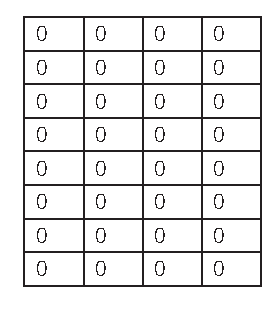
\includegraphics[width=.4\textwidth]{绘图2.eps}    %xx.eps是图片文件的相对路径
	\caption{初始状态}                                  %图片的标题
	\label{img}                                     %此处的label相当于一个图片的专属标志,目的是方便上下文的引用
\end{figure}
当j=n时,空字符串是任何字符串的子序列,所以dp[i][n]=1
\begin{figure}[H]
	\centering                                      %图片居中
	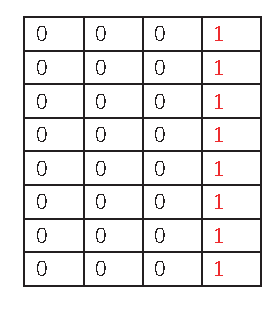
\includegraphics[width=.4\textwidth]{绘图3.eps}    %xx.eps是图片文件的相对路径
	\caption{dp[i][n]=1}                                  %图片的标题
	\label{img}                                     %此处的label相当于一个图片的专属标志,目的是方便上下文的引用
\end{figure}
计算dp[6][2]:s[i]=t[j]=g,所以dp[i][j]=dp[i+1][j+1]+dp[i+1][j]
\begin{figure}[H]
	\centering                                      %图片居中
	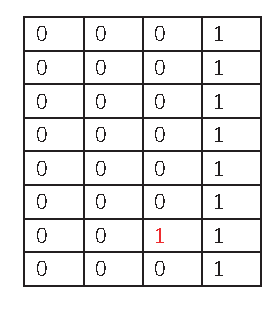
\includegraphics[width=.4\textwidth]{绘图4.eps}    %xx.eps是图片文件的相对路径
	\caption{dp[6][2]=dp[7][3]+dp[7][2]=1}                                  %图片的标题
	\label{img}                                     %此处的label相当于一个图片的专属标志,目的是方便上下文的引用
\end{figure}
计算dp[6][1]:s[i]=g而t[j]=a,两者不相等,所以dp[i][j]=dp[i+1][j]
\begin{figure}[H]
	\centering                                      %图片居中
	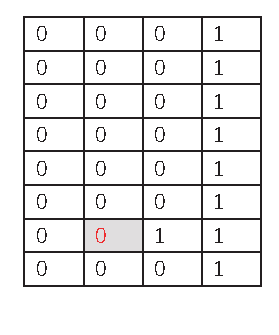
\includegraphics[width=.4\textwidth]{绘图5.eps}    %xx.eps是图片文件的相对路径
	\caption{dp[6][1]=dp[7][1]=0}                                  %图片的标题
	\label{img}                                     %此处的label相当于一个图片的专属标志,目的是方便上下文的引用
\end{figure}
其他位置同理,此处省略。
最终:
\begin{figure}[H]
	\centering                                      %图片居中
	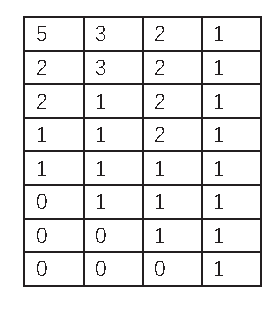
\includegraphics[width=.4\textwidth]{绘图6.eps}    %xx.eps是图片文件的相对路径
	\caption{最终结果返回dp[0][0]=5}                                  %图片的标题
	\label{img}                                     %此处的label相当于一个图片的专属标志,目的是方便上下文的引用
\end{figure}
和预测结果一样,最终结果为5。
\subsection{Analysis of Complexity}
时间复杂度$O(mn)$,m,n分别是字符串s和t的长度,二维数组dp有m+1行和n+1列,需对dp中每个元素进行计算,所以时间复杂度为$O(mn)$。
空间复杂度也为$O(mn)$,因为创建了m+1行n+1列的二维数组dp[i][j]。

\end{homeworkProblem}

\end{document}